%==============================================================
% AJOUTS A INSERER DANS main.tex
% Objectif : ajouter uniquement les 2 logos et les screenshots.
%==============================================================

%--------------------------------------------------------------
% 1) A ajouter apres \usepackage{graphicx}
%--------------------------------------------------------------
\graphicspath{{assets/}}

%--------------------------------------------------------------
% 2) Dans la page de garde, juste apres \begin{center}
%--------------------------------------------------------------
\begin{minipage}{0.45\textwidth}
  \raggedright
  
\includegraphics[width=0.82\linewidth]{logo_ehtp.png}
\end{minipage}
\hfill
\begin{minipage}{0.45\textwidth}
  \raggedleft
  
\includegraphics[width=0.95\linewidth]{logo_bvc.png}
\end{minipage}

\vspace{0.8cm}

% Option conseillee : remplacer la ligne
% \newcommand{\etablissement}{[Votre \'{E}cole / Universit\'{e}]}
% par :
% \newcommand{\etablissement}{Ecole Hassania des Travaux Publics}

%--------------------------------------------------------------
% 3) Section a ajouter dans "Presentation des Tableaux de Bord"
%    idealement juste apres :
%    \section{Presentation des Tableaux de Bord}
%--------------------------------------------------------------
\subsection{Captures reelles de l'application Streamlit}

Les captures suivantes presentent les principales pages de
l'application developpee. Elles illustrent le passage des resultats
du pipeline analytique vers une interface exploitable par les equipes
metier : synthese marche, analyse par instrument, centre d'alertes,
vue Machine Learning et import de donnees.

\begin{figure}[H]
\centering
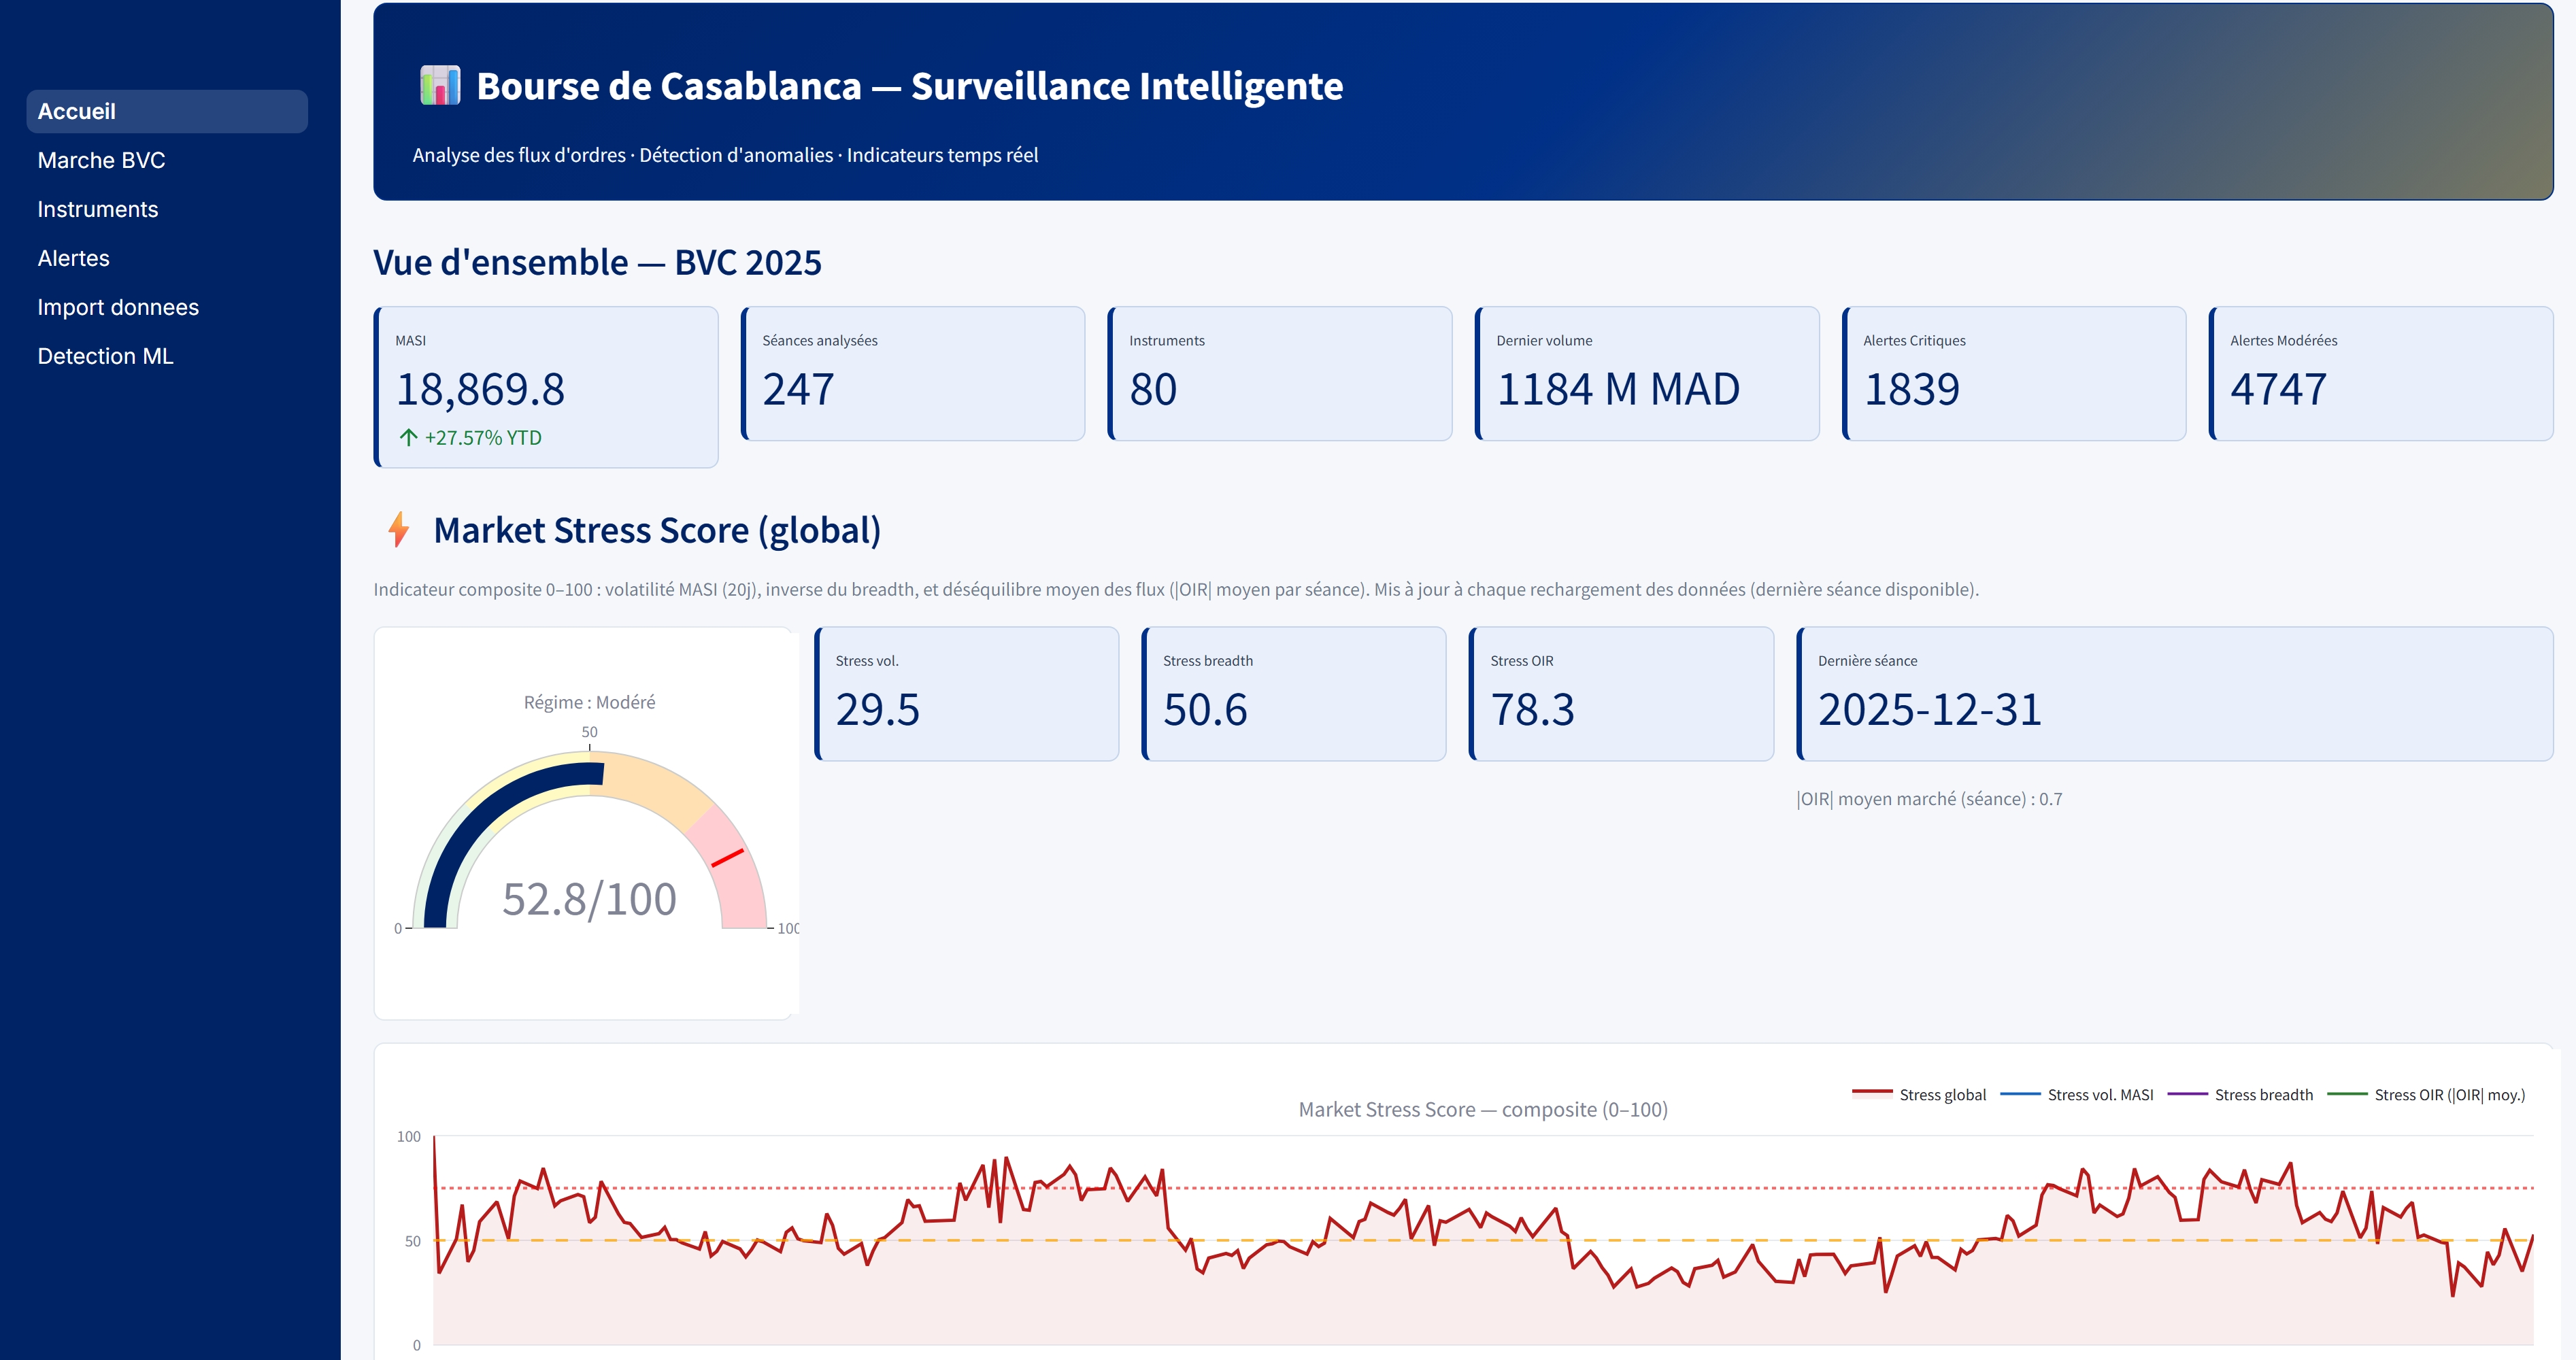
\includegraphics[width=0.95\textwidth]{screen_accueil.jpeg}
\caption{Page Accueil --- Synthese BVC 2025 : KPIs de marche, nombre de seances analysees, instruments suivis, alertes critiques et score de stress global.}
\label{fig:screen_accueil}
\end{figure}

La page d'accueil joue le role de tableau de bord executif. Elle
resume l'etat du marche a travers le MASI, les volumes, le nombre
d'instruments, les alertes critiques et moderees, ainsi que le score
de stress global. Ce score permet d'identifier rapidement si le marche
presente un regime normal, modere ou tendu.

\begin{figure}[H]
\centering
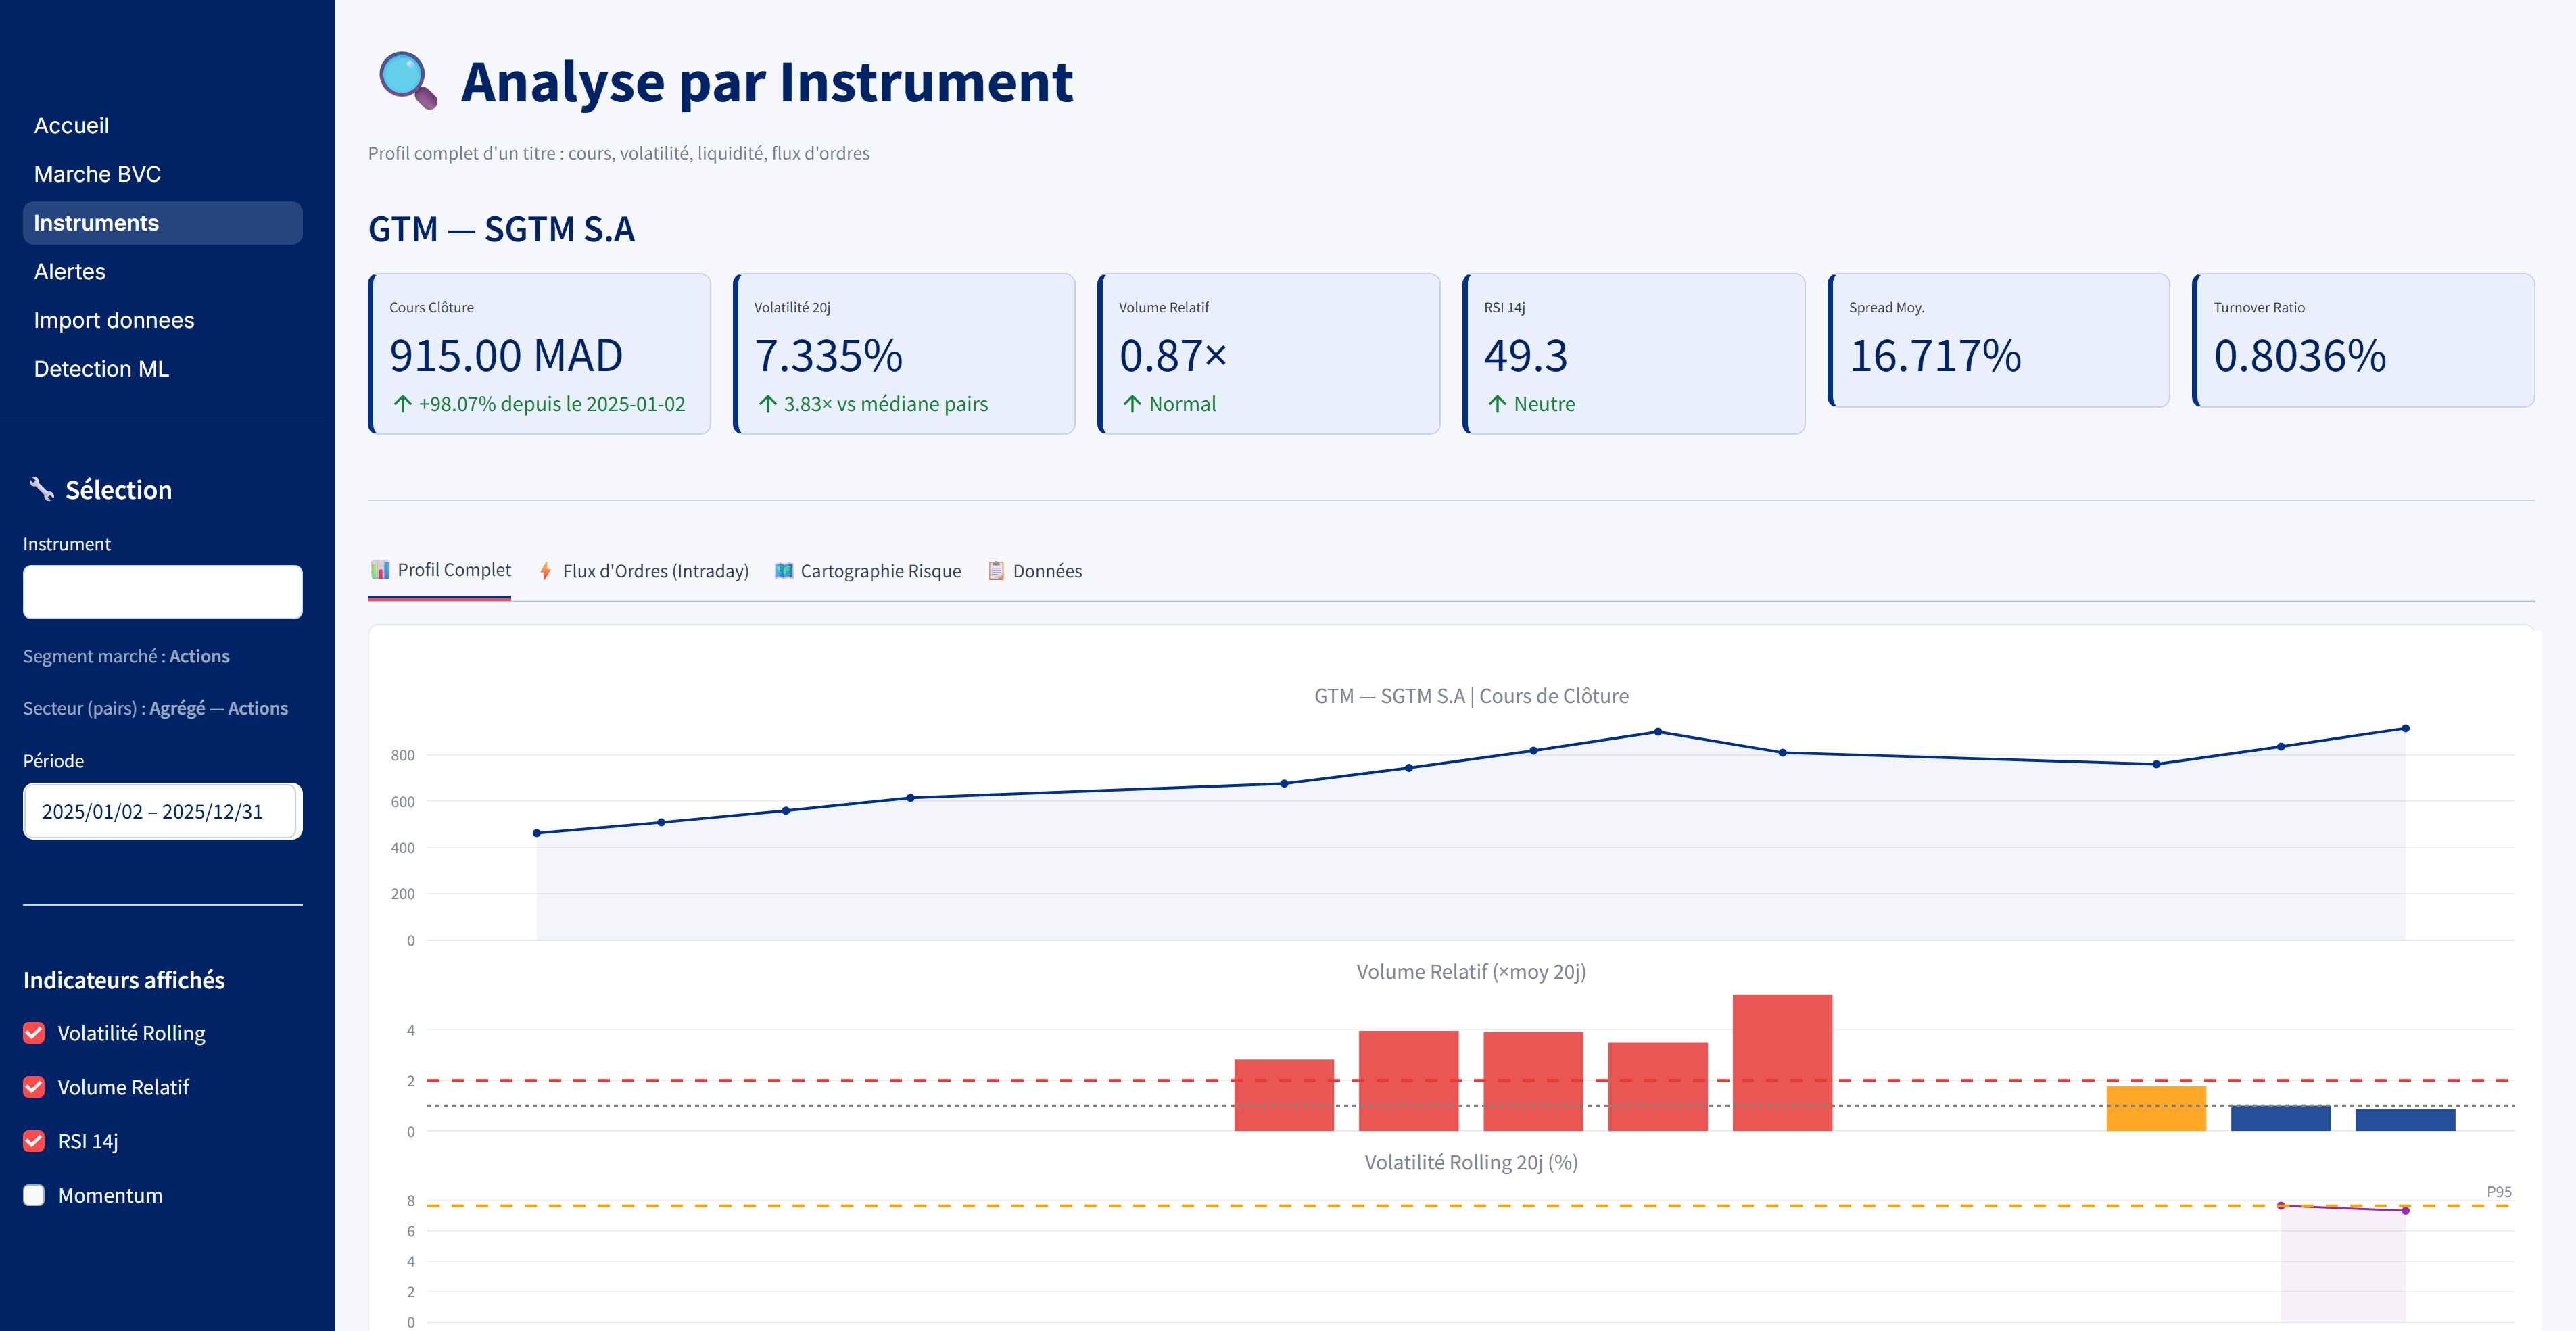
\includegraphics[width=0.95\textwidth]{screen_instrument.jpeg}
\caption{Page Instruments --- Analyse detaillee d'un titre : cours, volatilite, volume relatif, RSI, spread moyen et turnover.}
\label{fig:screen_instrument}
\end{figure}

La page d'analyse par instrument permet d'isoler un titre et
d'observer ses indicateurs propres. Elle aide a distinguer une alerte
liee au comportement general du marche d'une alerte propre a un
instrument : hausse de volatilite, volume relatif anormal, degradation
du spread ou signal de momentum.

\begin{figure}[H]
\centering
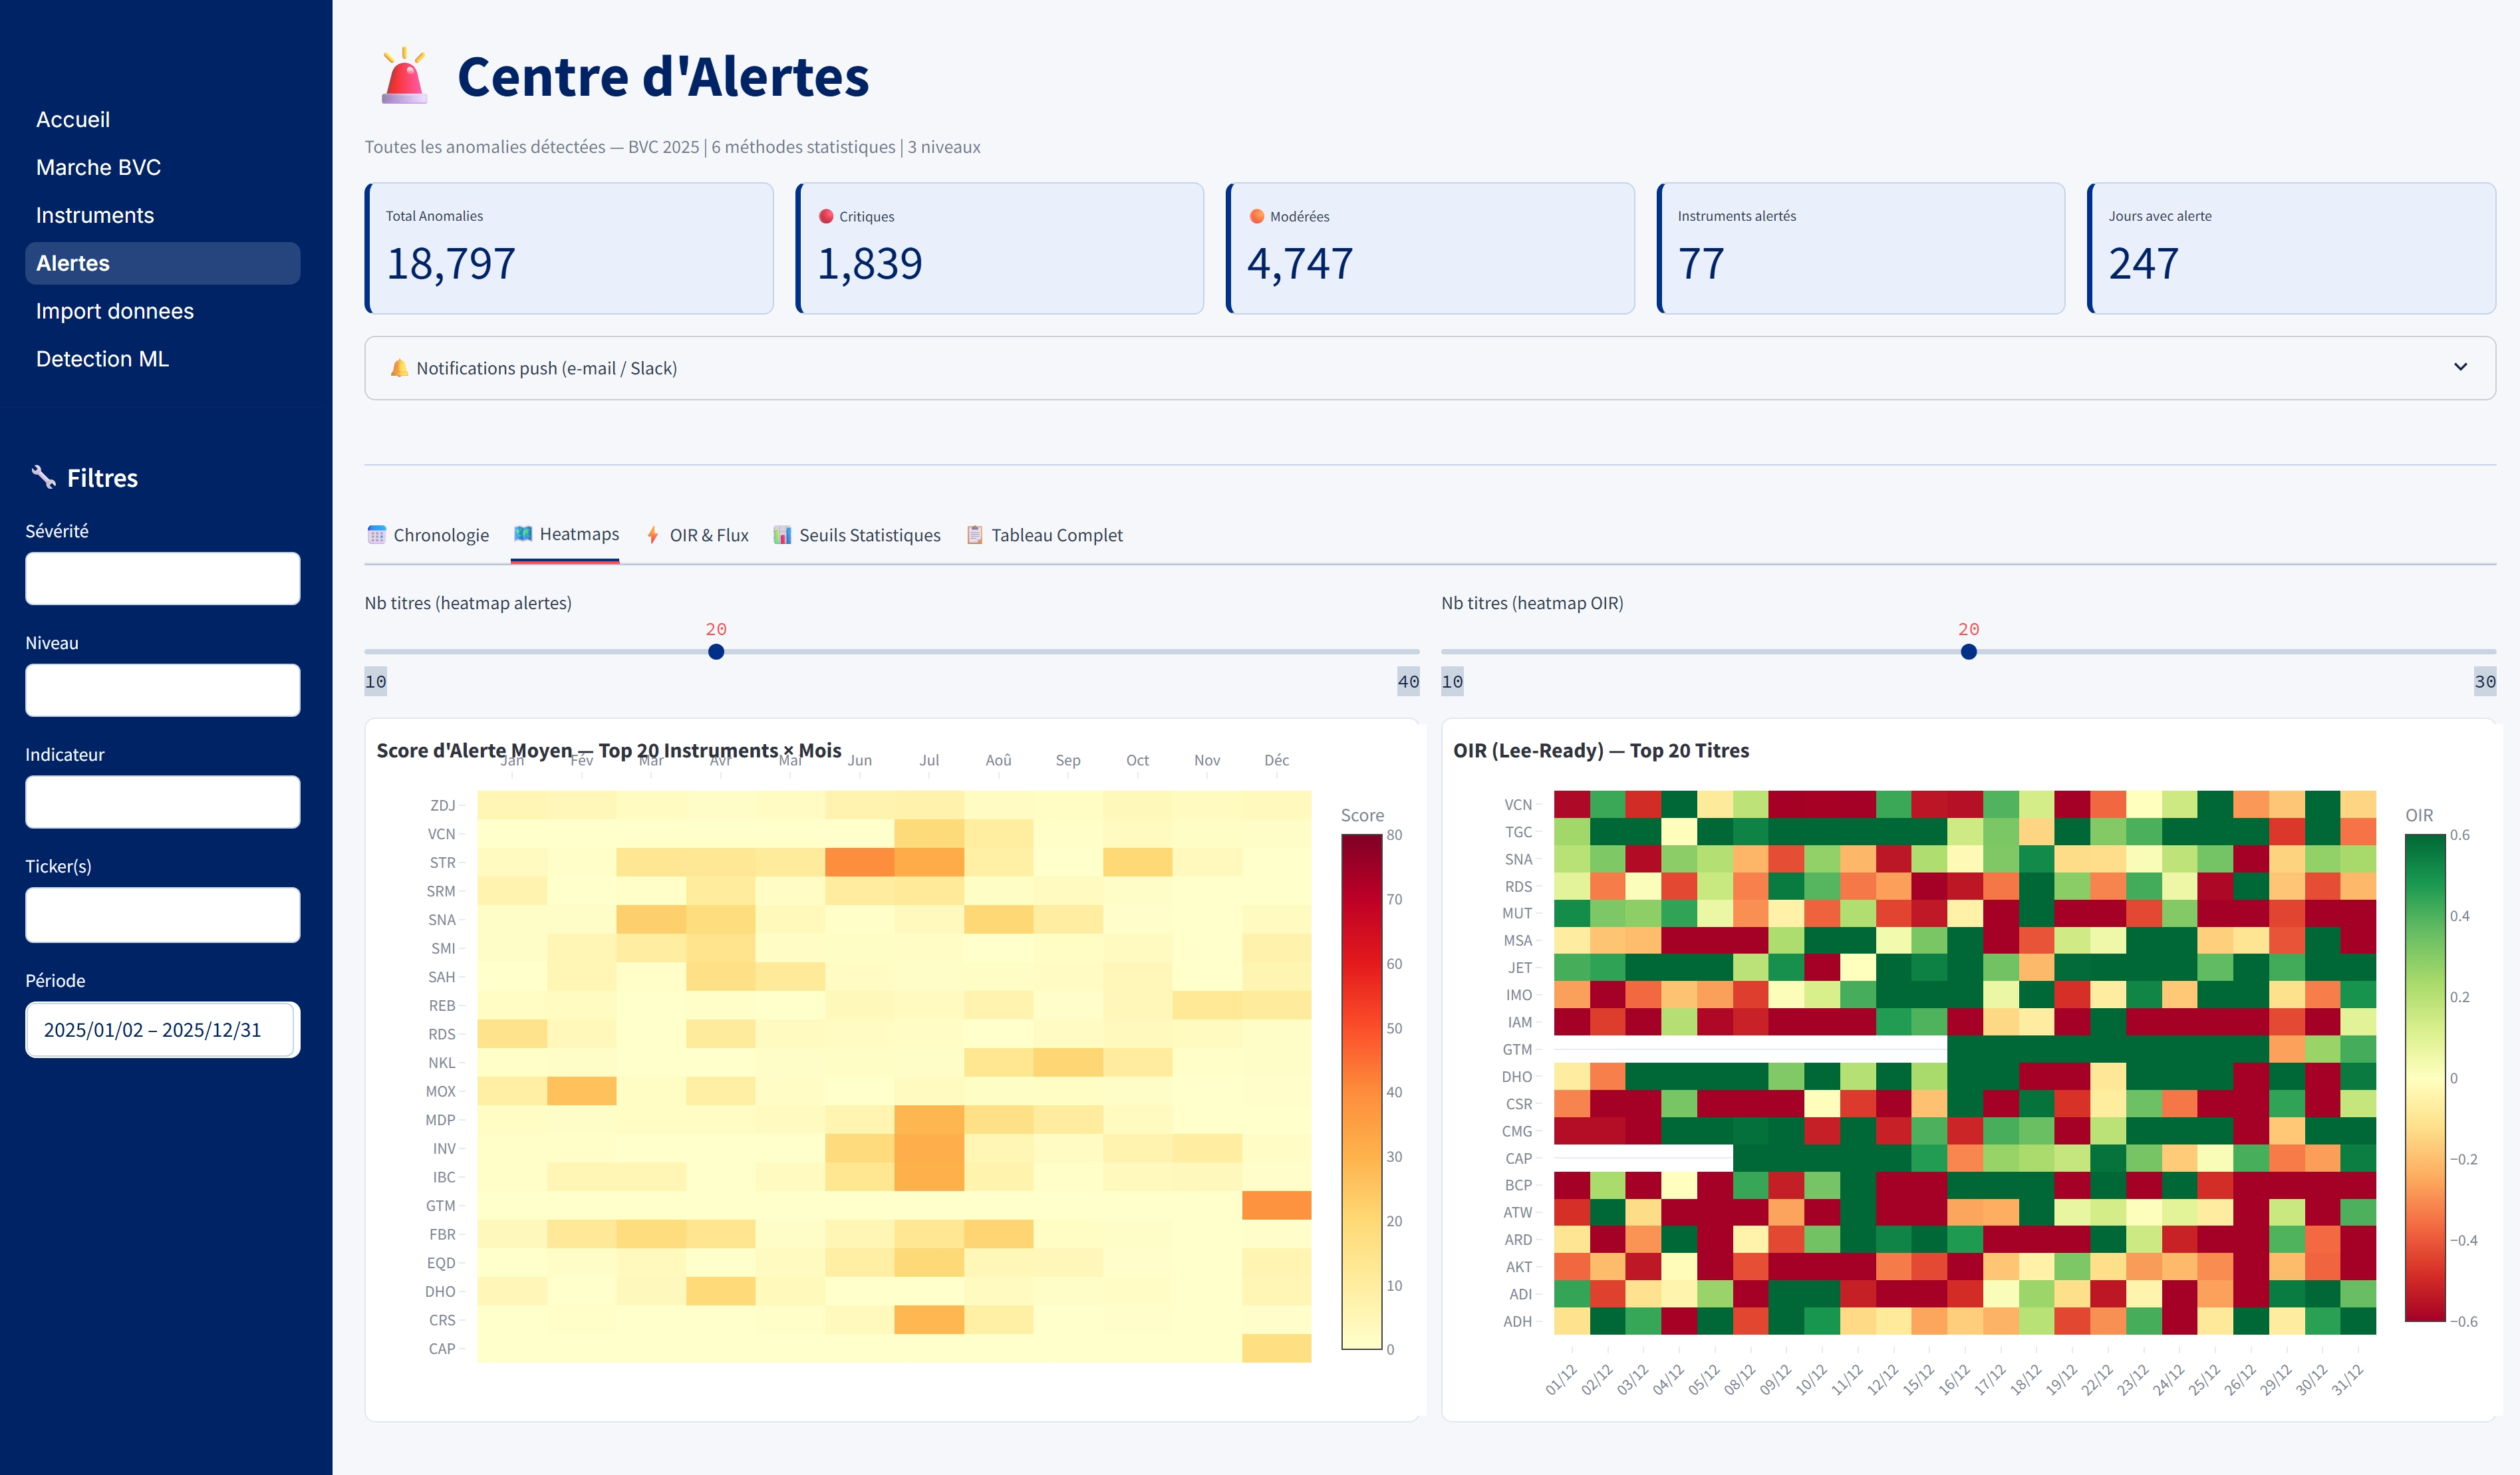
\includegraphics[width=0.95\textwidth]{screen_alertes_heatmap.jpeg}
\caption{Centre d'alertes --- Vue consolidee des anomalies : filtres, KPIs d'alertes et heatmaps par instrument et periode.}
\label{fig:screen_alertes}
\end{figure}

Le centre d'alertes constitue la vue operationnelle principale. Les
anomalies peuvent etre filtrees par severite, niveau, indicateur,
ticker et periode. Les heatmaps facilitent l'identification des
instruments et des mois concentrant les signaux les plus importants.

\begin{figure}[H]
\centering
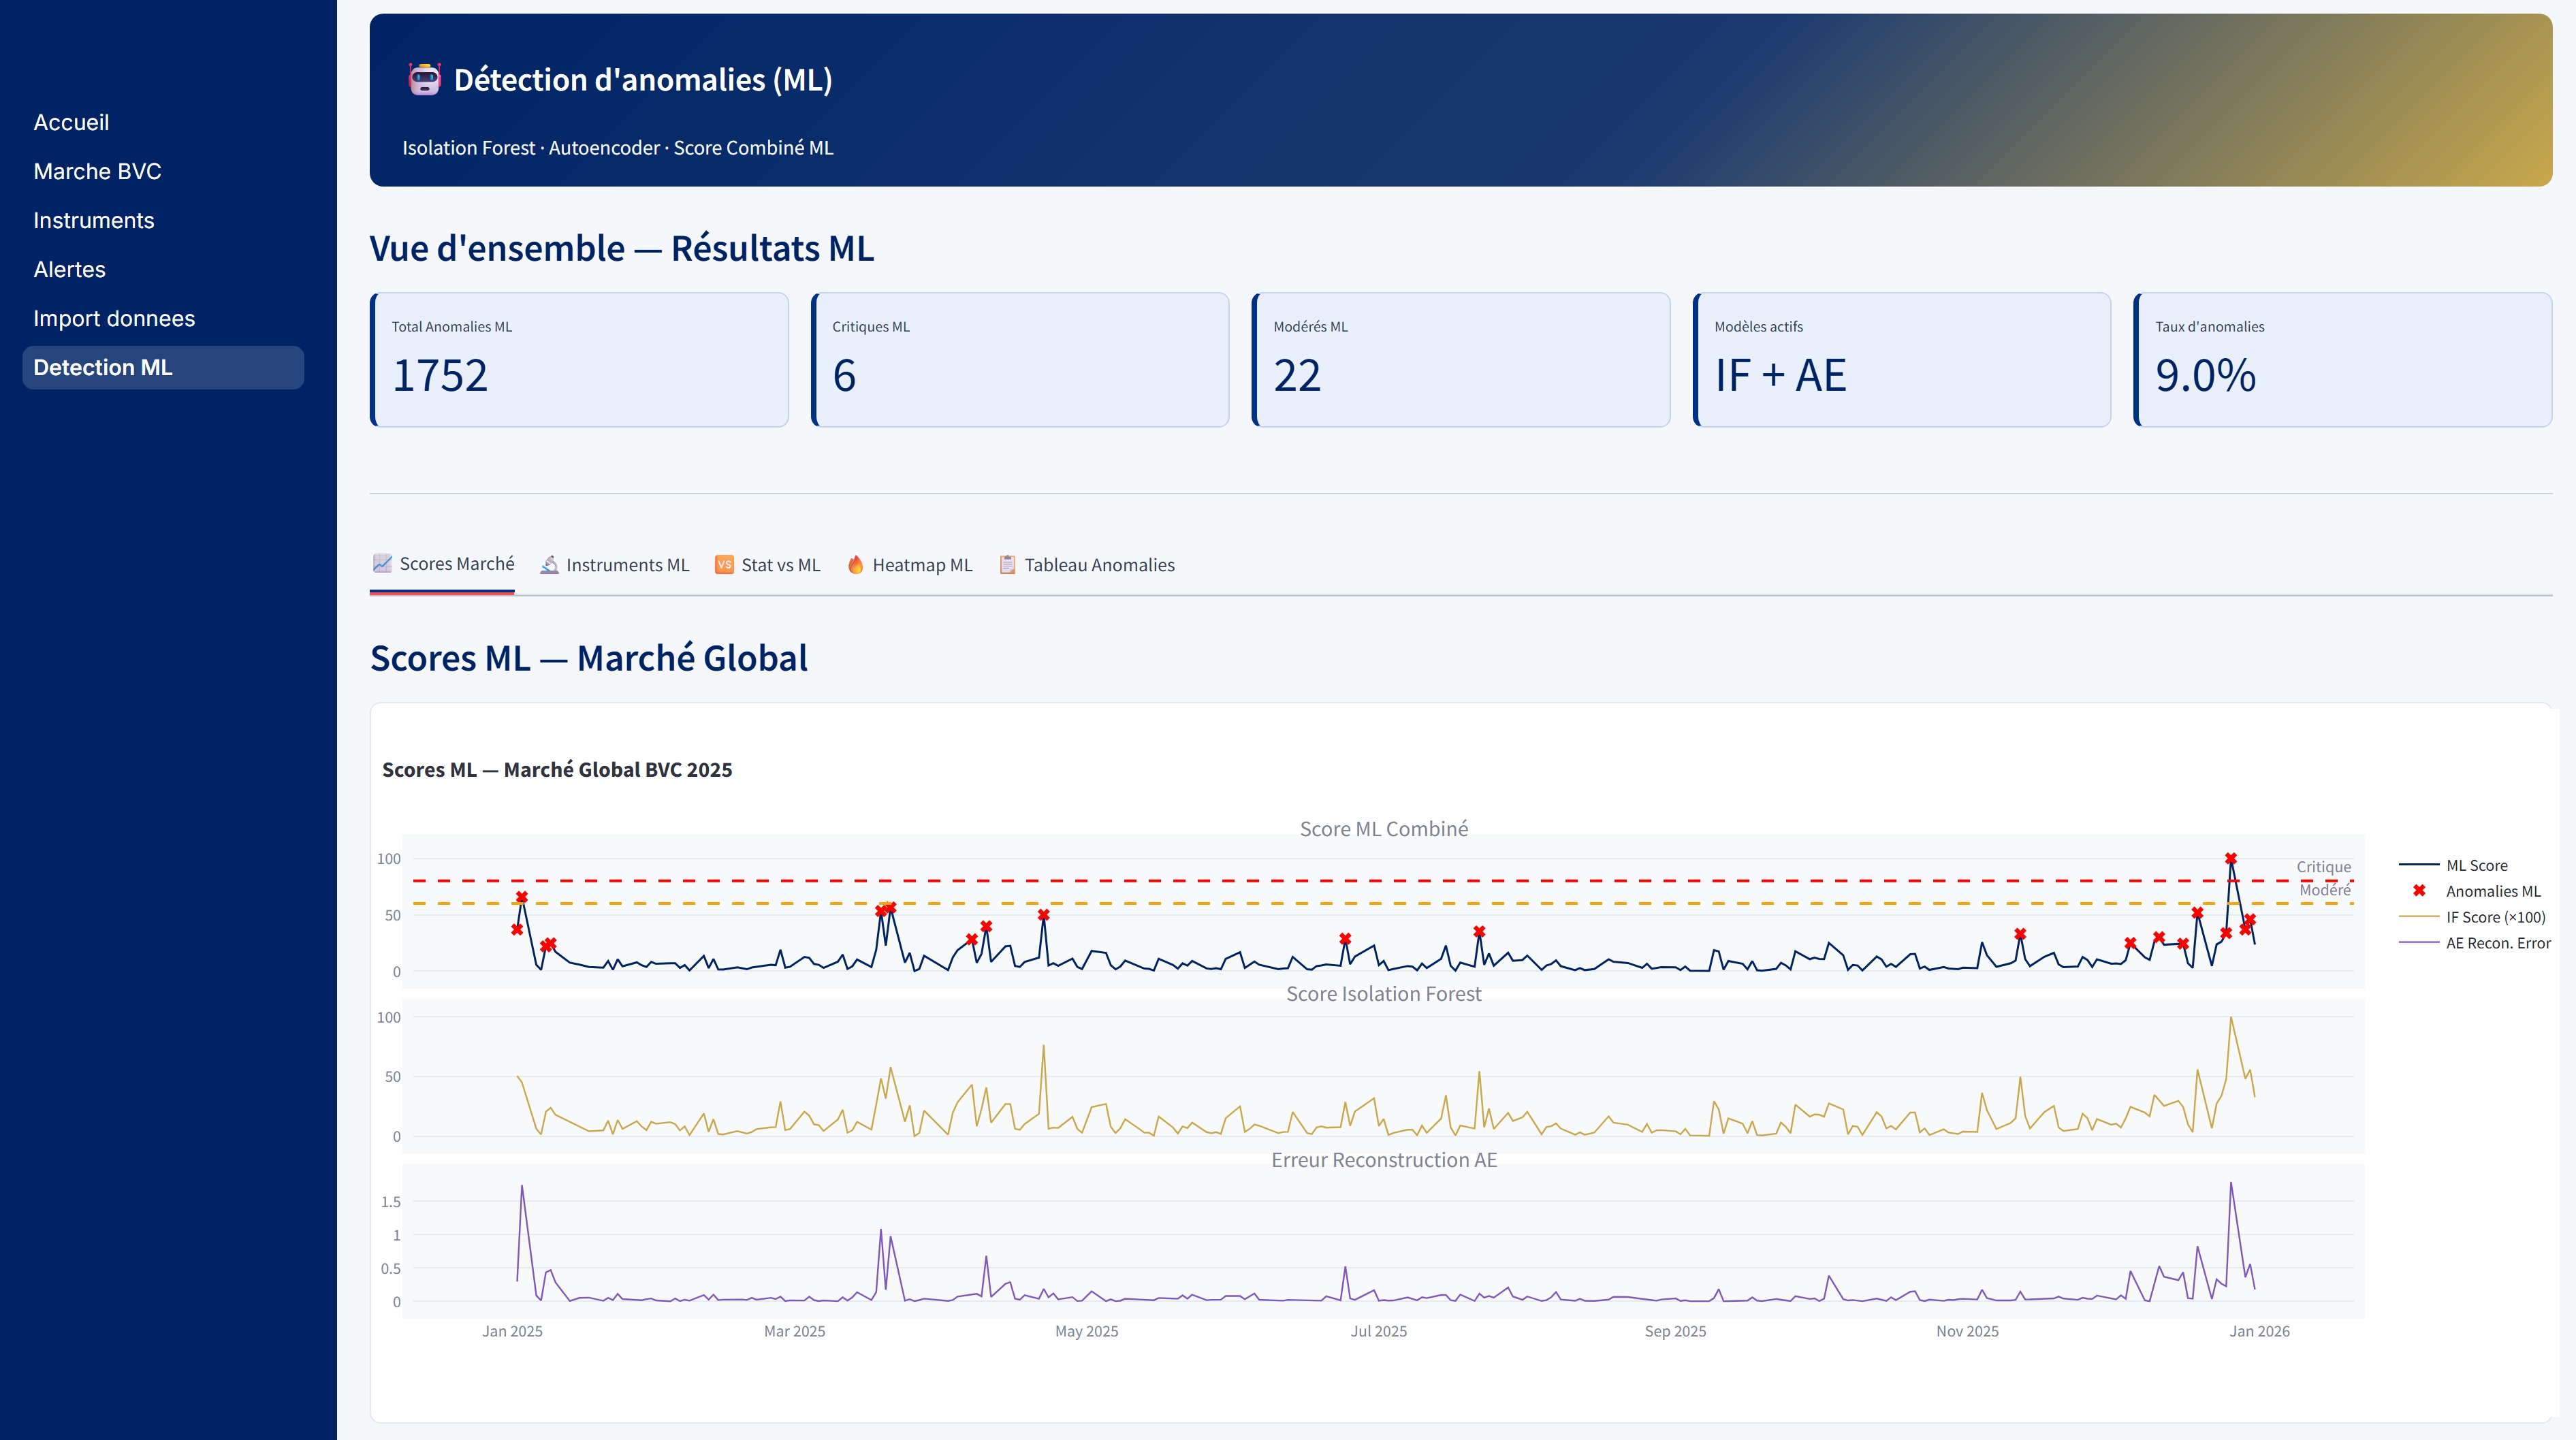
\includegraphics[width=0.95\textwidth]{screen_ml_global.jpeg}
\caption{Page Detection ML --- Resultats des modeles non supervises : Isolation Forest, Autoencoder et score ML combine.}
\label{fig:screen_ml}
\end{figure}

La page de detection ML compare les signaux issus de l'Isolation
Forest et de l'Autoencoder. Le score combine permet de reperer les
observations atypiques qui ne sont pas toujours detectees par une
seule regle statistique.

\begin{figure}[H]
\centering
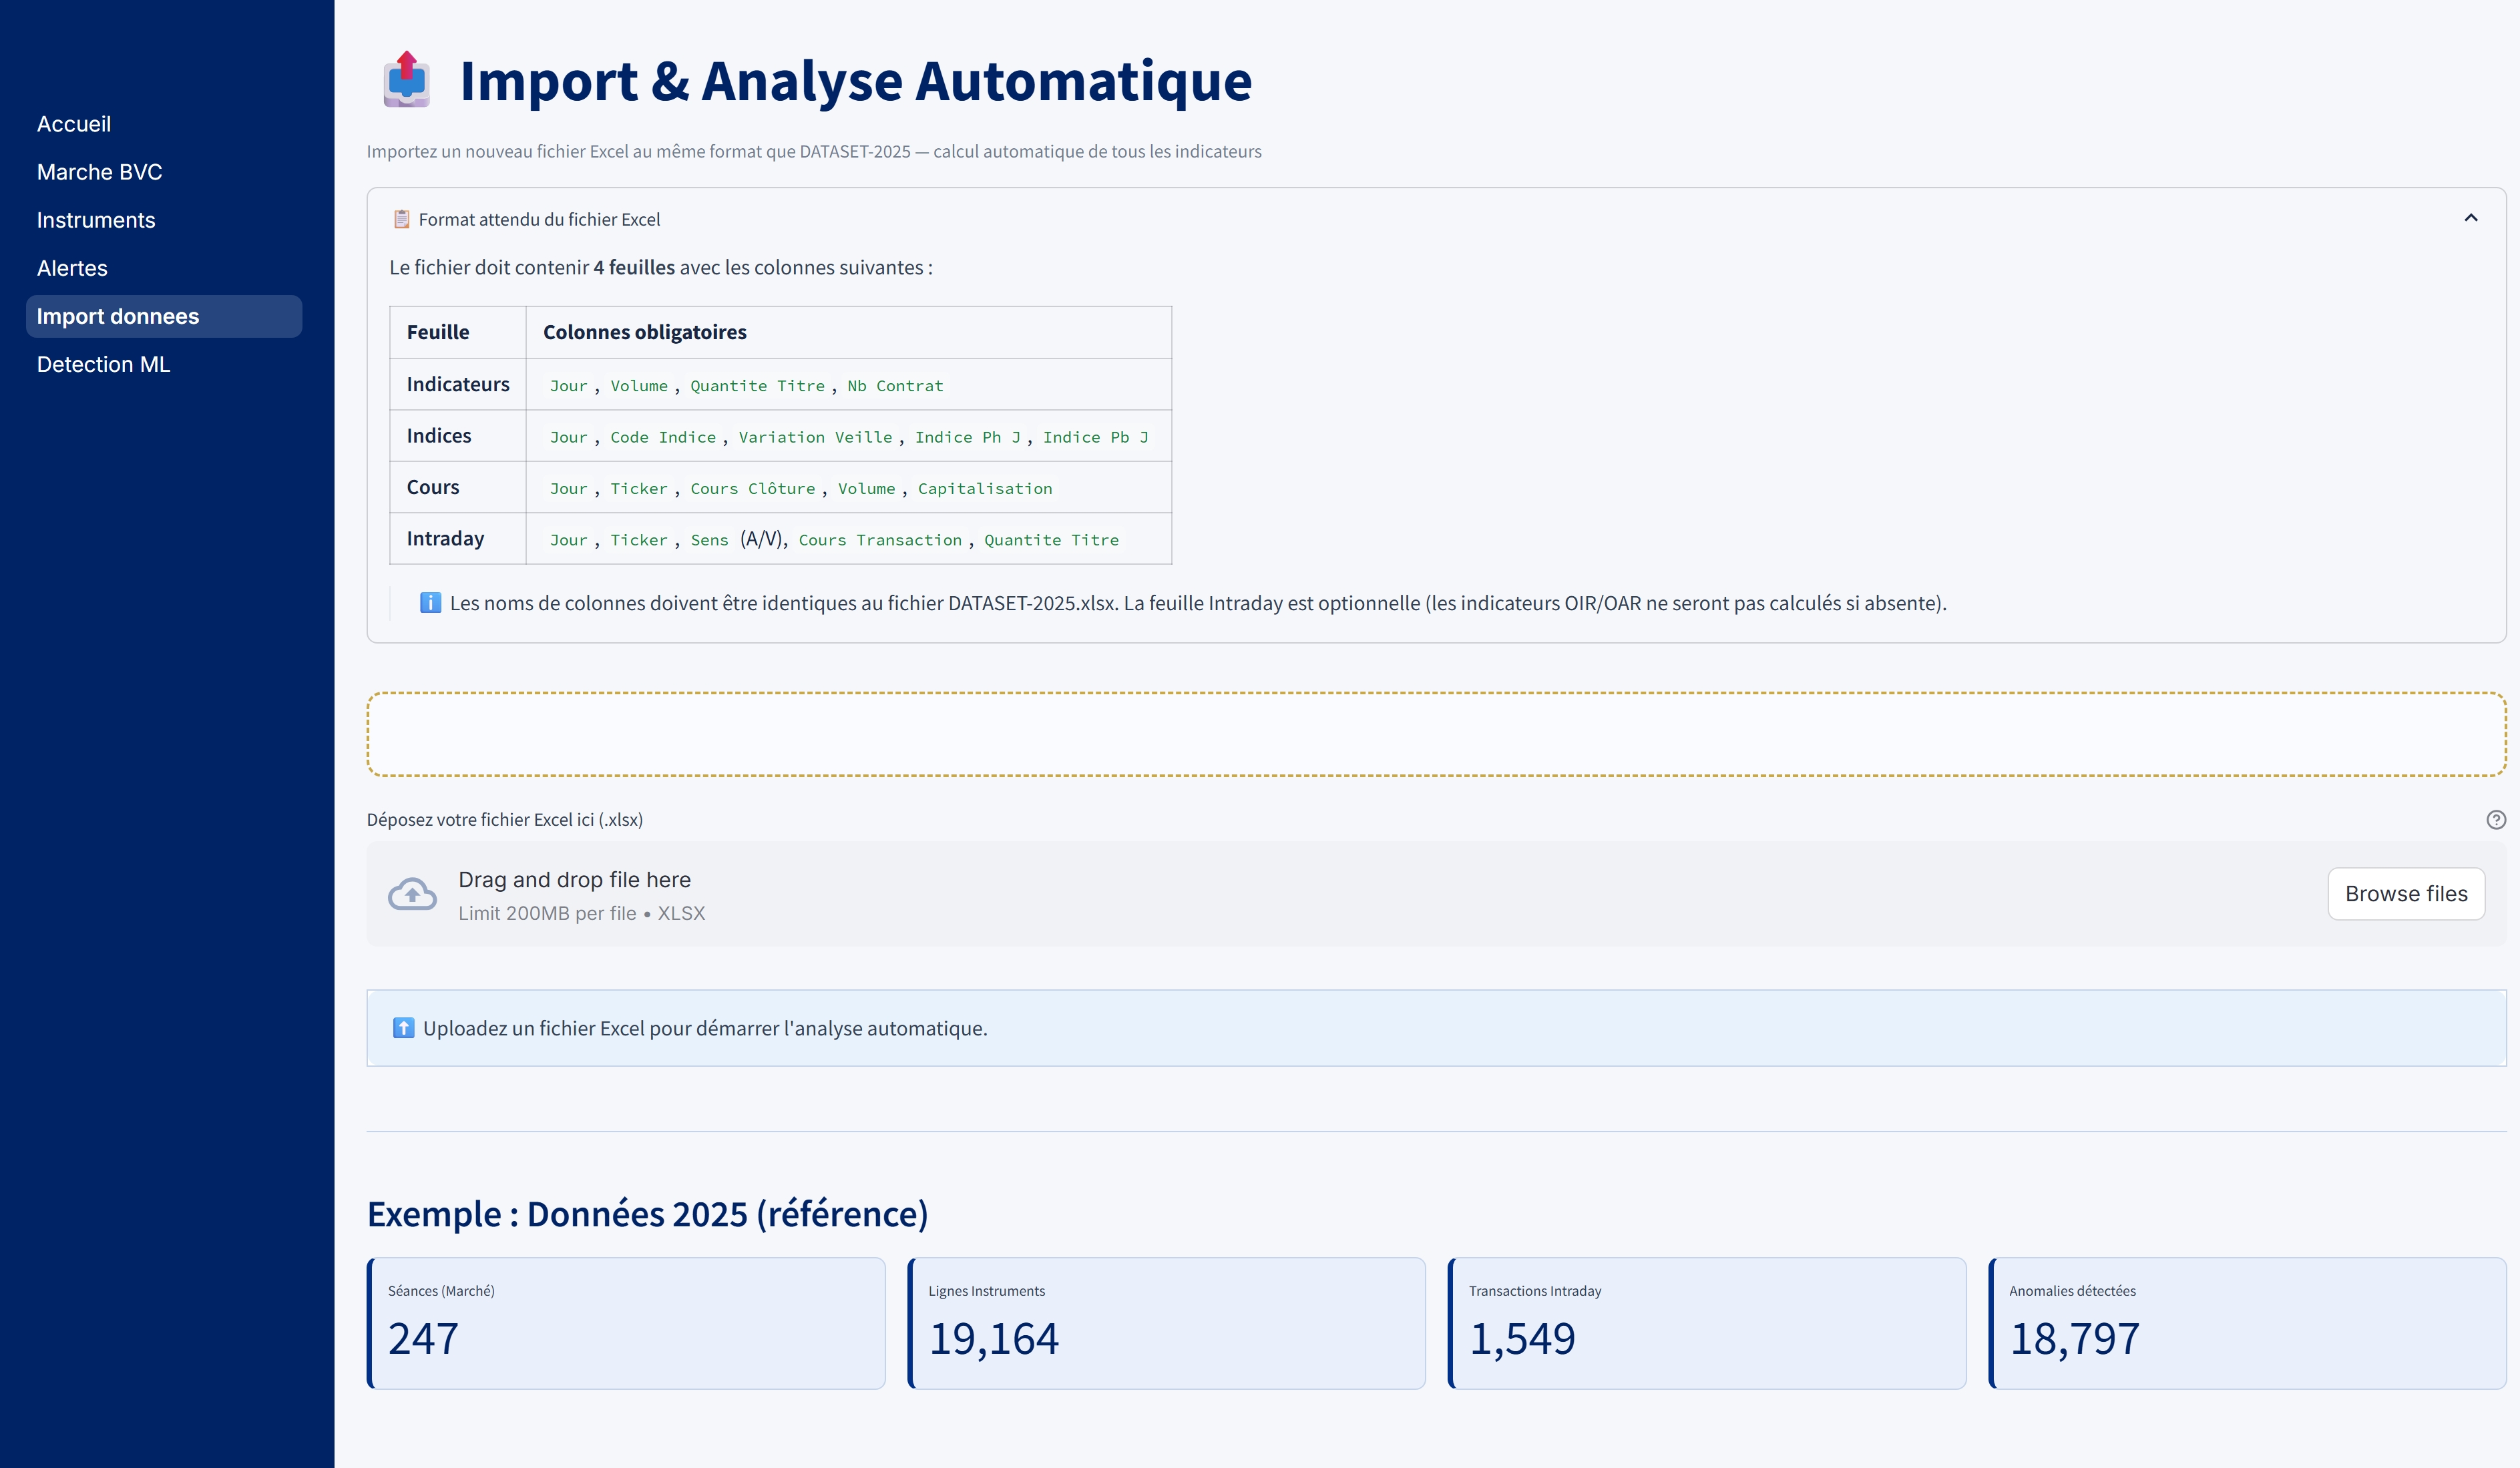
\includegraphics[width=0.95\textwidth]{screen_import.jpeg}
\caption{Page Import donnees --- Chargement d'un fichier Excel, validation du format et relance automatique du pipeline.}
\label{fig:screen_import}
\end{figure}

La page d'import rend le systeme reutilisable. Un nouveau fichier
Excel respectant le format attendu peut etre charge, valide, puis
traite pour recalculer les indicateurs, les scores d'alerte et les
anomalies sans intervention directe dans le code source.

